\documentclass{article}
\usepackage[utf8]{inputenc}
\usepackage[top=0.75in, bottom=0.75in, left=0.65in, right=0.65in]{geometry}
\usepackage{graphicx}
\usepackage{amsmath}
\usepackage{amsmath}
\usepackage{amssymb}
\usepackage{listings}
\usepackage[T1]{fontenc}
\usepackage[lighttt]{lmodern}
\usepackage{filecontents}       % For the example data
\usepackage{pgfplotstable}
\usepackage{array}      % For aligining at decimal point
\usepackage{siunitx}
\usepackage{booktabs}

\usepackage{xcolor}
 
\definecolor{codegreen}{rgb}{0,0.6,0}
\definecolor{codegray}{rgb}{0.5,0.5,0.5}
\definecolor{codepurple}{rgb}{0.58,0,0.82}
\definecolor{backcolour}{rgb}{0.95,0.95,0.92}
 
\lstdefinestyle{mystyle}{
    backgroundcolor=\color{white},   
    commentstyle=\color{codegreen},
    keywordstyle=\color{magenta},
    numberstyle=\tiny\color{codegray},
    stringstyle=\color{codepurple},
    basicstyle=\ttfamily\footnotesize,
    breakatwhitespace=false,         
    breaklines=true,                 
    captionpos=b,                    
    keepspaces=true,                 
    numbers=left,                    
    numbersep=5pt,                  
    showspaces=false,                
    showstringspaces=false,
    showtabs=false,                  
    tabsize=2
}

\lstset{style=mystyle}
\usepackage{graphicx}
\graphicspath{{figure/}}


\newcommand*\lstinputpath[1]{\lstset{inputpath=#1}}
\lstinputpath{codes}
\title{Home Work 03: EAS 520}
\author{Sayem Khan}
\date{Tuesday, Nov 07, 2019}

\begin{document}

\maketitle
\subsection*{Task 1}
\subsubsection*{Problem a, b} 
Implementation of Monte Carlo integration algorithm in C, C++ or Fortran.
\subsubsection*{Solution}
The problem is given below:
\lstinputlisting[
  language   = C++,
  basicstyle = \ttfamily,
  frame      = single,
  caption    = {Code for Task 01},
]{mc10d_1_b.cpp}

\lstinputlisting[
  language = bash,
  basicstyle = \ttfamily,
  frame      = single,
  caption    = {Driver script for Task 01},
]{driver.sh}
For the problem output is taken for every $4^k$ step. Time using C++ time for the Serial code time for $N = 1000000000$ is $108.965s$. Also, same as the Linux timer that is \textbf{real 1m48.965s}. These result is documented in \textbf{dataSerial.dat} and \textbf{timedata.dat} files.
\lstinputlisting[
  language   = C++,
  basicstyle = \ttfamily,
  frame      = single,
  caption    = {Output sample for program},
]{dataSerial.dat}

\lstinputlisting[
  %language   = C++,
  basicstyle = \ttfamily,
  frame      = single,
  caption    = {Time, measured by C++ timer},
]{timeData.dat}
\begin{figure}[h!]
  \centering
    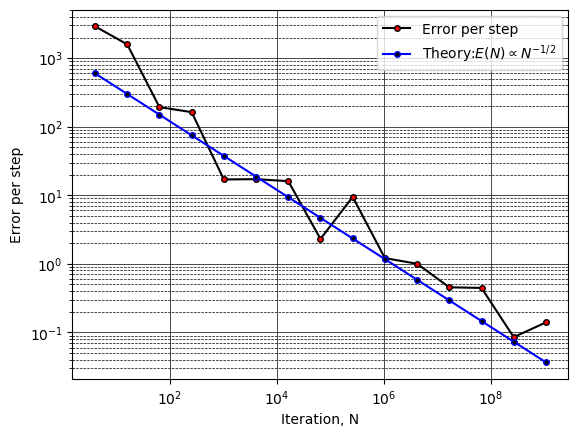
\includegraphics[width=0.85\textwidth]{step_by_step_error}
    \caption{Step by step error (For every $4^k$ step) and Theoretical Error for 10D MC integration for serial code. Error is decreasing, so we can say code is working properly.} 
    \label{t1a}
\end{figure}



\subsection*{Task 2}
\subsubsection*{Problem a}
 Use OpenMP to parallelize the for-loop over the number of N random samples.
 \subsubsection*{Solution}
\lstinputlisting[
  language   = C++,
  basicstyle = \ttfamily,
  frame      = single,
  caption    = {Code for Task 02, problem a (Prallel code for 10D integration)},
]{mc10d_parallel_2_a.cpp}
\lstinputlisting[
 % language   = C++,
  basicstyle = \ttfamily,
  frame      = single,
  caption    = {Output file for Task 02, problem a (dataParallel\_2\_a.dat). NB: Output pattern: "N Intergration wallTime MaxNumThread"},
]{dataParallel_2_a.dat}

\subsubsection*{Problem b}
Parallel code for output every $4^k$  step. 
 \subsubsection*{Solution}
\lstinputlisting[
  language   = C++,
  basicstyle = \ttfamily,
  frame      = single,
  caption    = {Code for Task 02, problem b (Prallel code for 10D integration with output for every $4^k$ step)},
]{mc10d_parallel_2_b.cpp}

\lstinputlisting[
 % language   = C++,
  %basicstyle = \ttfamily,
  frame      = single,
  caption    = {Output file for Task 02, problem b (dataParallel\_2\_b.dat). Master thread did the final work.},
]{dataParallel_2_b.dat}

\subsubsection*{Problem c}
Time for both serial and parallel code.
 \subsubsection*{Solution}
 Driver program is given below:
 \lstinputlisting[
  language = bash,
  basicstyle = \ttfamily,
  frame      = single,
  caption    = {Driver script for Task 02, problem c},
]{driverTime.sh}
 Output is given below:
  \lstinputlisting[
  %language = bash,
  basicstyle = \ttfamily,
  frame      = single,
  caption    = {Times taken by Serial code},
]{timeSerial.dat}
  \lstinputlisting[
  %language = bash,
  basicstyle = \ttfamily,
  frame      = single,
  caption    = {Times taken by Parallel code},
]{timeParallel.dat}
Astonishingly, parallel code takes much time than Serial code. Since this program is run in my Laptop, it could be the effect of OS noise.
\begin{figure}[h!]
  \centering
    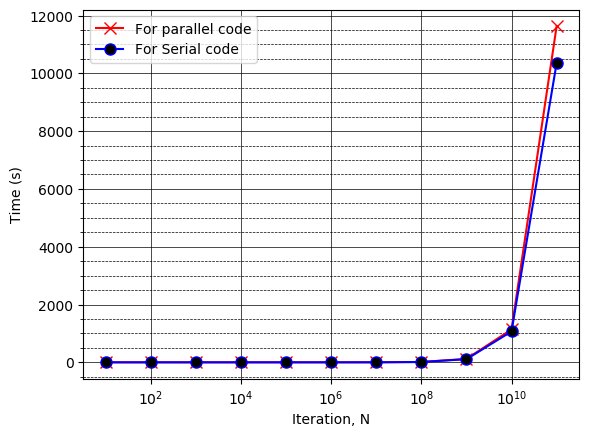
\includegraphics[width=0.6\textwidth]{Comparison_between_serial_and_parallel_times}
    \caption{Time comparison between Serial and Parallel code.} 
    \label{t1a}
\end{figure}



\subsubsection*{Problem d}
Comparison between Serial and parallel code.
 \subsubsection*{Solution}
\begin{figure}[h!]
  \centering
    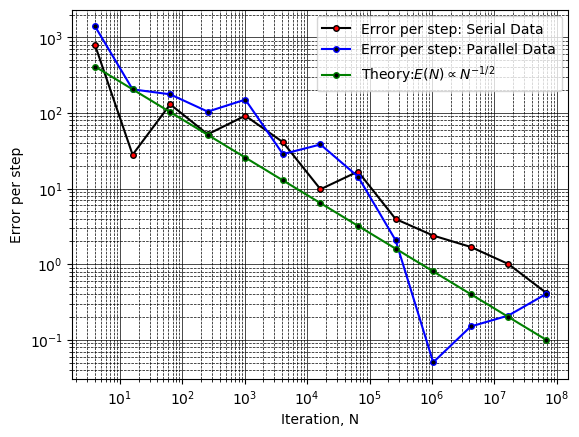
\includegraphics[width=0.6\textwidth]{Comparison_between_serial_and_parallel.png}
    \caption{Step by step error (For every $4^k$ step) and Theoretical Error for 10D MC integration for serial code and Parallel. Error is decreasing, so we can say code is working properly.} 
   % \label{t1a}
\end{figure}

\begin{figure}[h!]
  \centering
    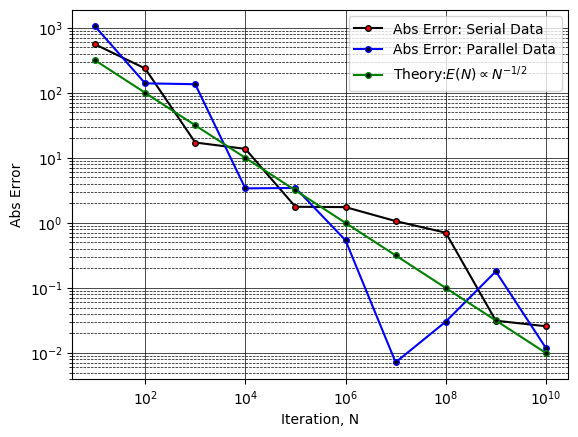
\includegraphics[width=0.6\textwidth]{Comparison_between_serial_and_parallel_1.png}
    \caption{Absolute Error and Theoretical Error for 10D MC integration for serial code and Parallel. Error is decreasing, so we can say code is working properly.} 
   % \label{t1a}
\end{figure}
\newpage
\subsection*{Task 3}
\subsubsection*{Problem a}
 Modification of OpenMP parallelized code to for Likelihood function.
\subsubsection*{Solution}
Code snippet for Task 3, problem a is given below:
\lstinputlisting[
  language   = C++,
  basicstyle = \ttfamily,
  frame      = single,
  caption    = {Code snippet for Task 3, problem a.},
]{3_a.cpp}
By using the driver program:
\lstinputlisting[
  language   = Bash,
  basicstyle = \ttfamily,
  frame      = single,
  caption    = {Driver program for Task 3, problem a},
]{3_a_driver.sh}

\lstinputlisting[
 % language   = Bash,
  basicstyle = \ttfamily,
  frame      = single,
  caption    = {Ouput of the program Task 3, problem a. Output pattern: N-Integration-wallTime-MaxNumThrea},
]{3_a_data.dat}

\subsubsection*{Problem b}
Testing the equation.
\subsubsection*{Solution}
If we out $x_i = 1$ we should get output like $\ln L = 0$, if we put $x_i = 0$ we should get output like $\ln L = -9$.
\lstinputlisting[
  language   = C++,
  basicstyle = \ttfamily,
  frame      = single,
  caption    = {Code snippet for Task 3, problem a.},
]{3_b.cpp}
Output is given below:
\lstinputlisting[
  %language   = C++,
  basicstyle = \ttfamily,
  frame      = single,
  caption    = {Testing the function.},
]{testFqnData.dat}

\subsubsection*{Problem c}
Scaling test.
\subsubsection*{Solution}
Scaling test is done in Stampede2. Every data is taken 100 times to minimize the noise.
\begin{figure}[h!]
  \centering
    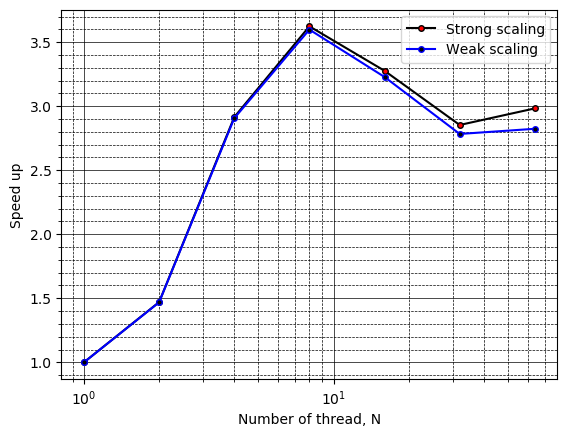
\includegraphics[width=0.8\textwidth]{3_c_scaling}
    \caption{Strong and weak scaling test.} 
    \label{t1a}
\end{figure}
Script is given below: 
\lstinputlisting[
  language   = Bash,
  basicstyle = \ttfamily,
  frame      = single,
  caption    = {Testing the function.},
]{3_c_stampede2.job}
\subsubsection*{Problem d}
Output of the integration after each $4^k$ step.
\subsubsection*{Solution}
The code is given below: 
\lstinputlisting[
  language   = C++,
  basicstyle = \ttfamily,
  frame      = single,
  caption    = {Code for Task 3, problem d.},
]{mc10d_parallel_3_d_1.cpp}
This code run on Stampede2. The script is given below: 
\lstinputlisting[
  language   = Bash,
  basicstyle = \ttfamily,
  frame      = single,
  caption    = {Code for Task 3, problem d.},
]{3_d_stampede2.job}
The output data is:
\lstinputlisting[
  language   = Bash,
  basicstyle = \ttfamily,
  frame      = single,
  caption    = {Output for Task 3, problem d. Format: N-Integration-ErrorPerStep. Line 19 indicates total N at final, total time taken (measured by omp timer) and total number of threads.},
]{3_d_out.dat}
1-digit accuracy is achieved at N = 268435456. 
\\
\\
The below code was run in my laptop (Intel Core i5-2.3GHz, 2-cores). It took more than 2 hours with N = 68719476736 and have not achieved any 1-digit accuracy. 
\lstinputlisting[
  language   = C++,
  basicstyle = \ttfamily,
  frame      = single,
  caption    = {Code for Task 3, problem d (An alternative approach).},
]{3_d_mine.cpp}

\lstinputlisting[
  language   = C++,
  basicstyle = \ttfamily,
  frame      = single,
  caption    = {Output for Task 3, problem d (An alternative approach).},
]{3_d_mine.dat}
I can not figure out the bug! N.B: I did not upload this code in bitbucket. 



\end{document}
